\documentclass[border=4pt]{standalone}

\usepackage{amsmath}
\usepackage{tikz}
\usepackage{mathdots}
\usepackage{yhmath}
\usepackage{cancel}
\usepackage{color}
\usepackage{siunitx}
\usepackage{array}
\usepackage{multirow}
\usepackage{amssymb}
\usepackage{gensymb}
\usepackage{tabularx}
\usepackage{booktabs}
\usetikzlibrary{fadings}
\usetikzlibrary{patterns}


\begin{document}
 


\tikzset{every picture/.style={line width=0.75pt}} %set default line width to 0.75pt        

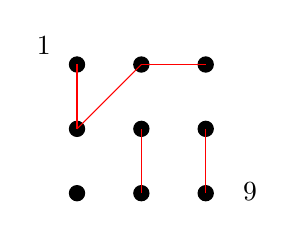
\begin{tikzpicture}[x=0.75pt,y=0.75pt,yscale=-1,xscale=1]
%uncomment if require: \path (0,300); %set diagram left start at 0, and has height of 300

%Shape: Circle [id:dp5291638232992628] 
\draw  [fill={rgb, 255:red, 0; green, 0; blue, 0 }  ,fill opacity=1 ] (75,126.33) .. controls (75,124.31) and (76.64,122.67) .. (78.67,122.67) .. controls (80.69,122.67) and (82.33,124.31) .. (82.33,126.33) .. controls (82.33,128.36) and (80.69,130) .. (78.67,130) .. controls (76.64,130) and (75,128.36) .. (75,126.33) -- cycle ;
%Shape: Circle [id:dp06751230716224854] 
\draw  [fill={rgb, 255:red, 0; green, 0; blue, 0 }  ,fill opacity=1 ] (75,64.33) .. controls (75,62.31) and (76.64,60.67) .. (78.67,60.67) .. controls (80.69,60.67) and (82.33,62.31) .. (82.33,64.33) .. controls (82.33,66.36) and (80.69,68) .. (78.67,68) .. controls (76.64,68) and (75,66.36) .. (75,64.33) -- cycle ;
%Shape: Circle [id:dp5585674722233964] 
\draw  [fill={rgb, 255:red, 0; green, 0; blue, 0 }  ,fill opacity=1 ] (106,64.33) .. controls (106,62.31) and (107.64,60.67) .. (109.67,60.67) .. controls (111.69,60.67) and (113.33,62.31) .. (113.33,64.33) .. controls (113.33,66.36) and (111.69,68) .. (109.67,68) .. controls (107.64,68) and (106,66.36) .. (106,64.33) -- cycle ;
%Shape: Circle [id:dp5063069448725839] 
\draw  [fill={rgb, 255:red, 0; green, 0; blue, 0 }  ,fill opacity=1 ] (75,95.33) .. controls (75,93.31) and (76.64,91.67) .. (78.67,91.67) .. controls (80.69,91.67) and (82.33,93.31) .. (82.33,95.33) .. controls (82.33,97.36) and (80.69,99) .. (78.67,99) .. controls (76.64,99) and (75,97.36) .. (75,95.33) -- cycle ;
%Shape: Circle [id:dp9693948917202144] 
\draw  [fill={rgb, 255:red, 0; green, 0; blue, 0 }  ,fill opacity=1 ] (106,95.33) .. controls (106,93.31) and (107.64,91.67) .. (109.67,91.67) .. controls (111.69,91.67) and (113.33,93.31) .. (113.33,95.33) .. controls (113.33,97.36) and (111.69,99) .. (109.67,99) .. controls (107.64,99) and (106,97.36) .. (106,95.33) -- cycle ;
%Shape: Circle [id:dp20822118405010004] 
\draw  [fill={rgb, 255:red, 0; green, 0; blue, 0 }  ,fill opacity=1 ] (106,126.33) .. controls (106,124.31) and (107.64,122.67) .. (109.67,122.67) .. controls (111.69,122.67) and (113.33,124.31) .. (113.33,126.33) .. controls (113.33,128.36) and (111.69,130) .. (109.67,130) .. controls (107.64,130) and (106,128.36) .. (106,126.33) -- cycle ;
%Shape: Circle [id:dp25687719289152877] 
\draw  [fill={rgb, 255:red, 0; green, 0; blue, 0 }  ,fill opacity=1 ] (137,64.33) .. controls (137,62.31) and (138.64,60.67) .. (140.67,60.67) .. controls (142.69,60.67) and (144.33,62.31) .. (144.33,64.33) .. controls (144.33,66.36) and (142.69,68) .. (140.67,68) .. controls (138.64,68) and (137,66.36) .. (137,64.33) -- cycle ;
%Shape: Circle [id:dp7962549519544571] 
\draw  [fill={rgb, 255:red, 0; green, 0; blue, 0 }  ,fill opacity=1 ] (137,95.33) .. controls (137,93.31) and (138.64,91.67) .. (140.67,91.67) .. controls (142.69,91.67) and (144.33,93.31) .. (144.33,95.33) .. controls (144.33,97.36) and (142.69,99) .. (140.67,99) .. controls (138.64,99) and (137,97.36) .. (137,95.33) -- cycle ;
%Shape: Circle [id:dp08538595729566989] 
\draw  [fill={rgb, 255:red, 0; green, 0; blue, 0 }  ,fill opacity=1 ] (137,126.33) .. controls (137,124.31) and (138.64,122.67) .. (140.67,122.67) .. controls (142.69,122.67) and (144.33,124.31) .. (144.33,126.33) .. controls (144.33,128.36) and (142.69,130) .. (140.67,130) .. controls (138.64,130) and (137,128.36) .. (137,126.33) -- cycle ;
%Straight Lines [id:da39504050319048356] 
\draw [color={rgb, 255:red, 255; green, 0; blue, 0 }  ,draw opacity=1 ]   (78.67,64.33) -- (78.67,95.33) ;


%Straight Lines [id:da5150914603150154] 
\draw [color={rgb, 255:red, 255; green, 0; blue, 0 }  ,draw opacity=1 ]   (109.67,64.33) -- (78.67,95.33) ;


%Straight Lines [id:da2226032951481478] 
\draw [color={rgb, 255:red, 255; green, 0; blue, 0 }  ,draw opacity=1 ]   (140.67,64.33) -- (109.67,64.33) ;


%Straight Lines [id:da00029150042656156394] 
\draw [color={rgb, 255:red, 255; green, 0; blue, 0 }  ,draw opacity=1 ]   (109.67,126.33) -- (109.67,95.33) ;


%Straight Lines [id:da6605153940581407] 
\draw [color={rgb, 255:red, 255; green, 0; blue, 0 }  ,draw opacity=1 ]   (140.67,126.33) -- (140.67,95.33) ;



% Text Node
\draw (62.67,55.33) node    {$1$};
% Text Node
\draw (162,125.67) node    {$9$};


\end{tikzpicture}

\end{document}
